%%%%%%%%%%%%%%%%%%%%%%%%%%%%%%%
\chapter{Field Class}

\section{BlockAttributes}
A block is a group of elements of identical shape, basis and order. The \lstinline[style=C++Style]!BlockAttributes! base class stores the most basic information of a block. The private member variables of the \lstinline[style=C++Style]!BlockAttributes! class are indicated below:

\begin{lstlisting}[style=C++Style]
class BlockAttributes
{   
public:
    BlockAttributes(const size_t num_elements,
                    const size_t num_elements_with_padding,
                    const size_t num_data, const size_t interleave_width)
        : m_num_elements(num_elements),
          num_elements_with_padding(num_elements_with_padding),
          m_num_data(num_data), m_size(num_elements_with_padding * num_data),
          m_interleave_width(interleave_width)
    {
    }
...

private:
    const size_t m_num_elements;
    const size_t num_elements_with_padding;
    const size_t m_num_data;
    const size_t m_size;
    size_t m_interleave_width;
};
\end{lstlisting}

Once a \lstinline[style=C++Style]!BlockAttributes! is instantiated, only the \lstinline[style=C++Style]!m_interleave_width! member variable can be modified by using the \lstinline[style=C++Style]!SetInterleaveWidth! member function
\begin{lstlisting}[style=C++Style]
void SetInterleaveWidth(const size_t interleave_width)
{
    ...
}
\end{lstlisting}


\section{BlockAccessor}
\lstinline[style=C++Style]!BlockAccessor! is a derived class of the \lstinline[style=C++Style]!BlockAttributes! base class. In addition of storing the basic information of a block, it also contains a reference to the \lstinline[style=C++Style]!MemoryRegion! object responsible of its memory management. An \lstinline[style=C++Style]!offset! member variable is also used to allow multiple blocks to map into a single \lstinline[style=C++Style]!MemoryRegion! as described later.

\begin{lstlisting}[style=C++Style]
template <typename TData> class BlockAccessor : public BlockAttributes
{
public:
    BlockAccessor(const BlockAttributes blockAttr,
                  MemoryRegion<TData> &memory_region, const size_t offset)
        : BlockAttributes(blockAttr), m_memory_region(memory_region),
          m_offset(offset)
    {
    }

    BlockAccessor(const size_t num_elements,
                  const size_t num_elements_with_padding, const size_t num_data,
                  const size_t interleave_width,
                  MemoryRegion<TData> &memory_region, const size_t offset)
        : BlockAttributes(num_elements, num_elements_with_padding, num_data,
                          interleave_width),
          m_memory_region(memory_region), m_offset(offset)
    {
    }

    ...
private:
    MemoryRegion<TData> &m_memory_region;
    size_t m_offset = 0;
};
\end{lstlisting}

Memory access to the private \lstinline[style=C++Style]!MemoryRegion! member variable is obtained through a templated \lstinline[style=C++Style]!GetPtr()! member function replicating the behavior of the \lstinline[style=C++Style]!MemoryRegion! class.  
\begin{lstlisting}[style=C++Style]
template <typename MemSpace, typename MemQualifier>
typename const_if<std::is_same_v<MemQualifier, ReadOnly>, TData>::type *GetPtr()
{
    return m_memory_region.template GetPtr<MemSpace, MemQualifier>() +
           m_offset;
}
\end{lstlisting}

Hence, various memory access mode of a \lstinline[style=C++Style]!BlockAccessor! object \lstinline[style=C++Style]!block! can be obtained as follow: 
\begin{lstlisting}[style=C++Style]
 auto ptr0 = block.template GetPtr<NektarSpaces::DeviceSpace, ReadOnly>;
 auto ptr1 = block.template GetPtr<NektarSpaces::DeviceSpace, WriteOnly>;
 auto ptr2 = block.template GetPtr<NektarSpaces::DeviceSpace, ReadWrite>;
\end{lstlisting}


\section{Field}
\subsection{Description}
A \lstinline[style=C++Style]!Field! is conceptually a list of blocks representing all the elements of a computational domain, where a block is a collection of elements of the same shape and order. The member variables of the \lstinline[style=C++Style]!Field! object are indicated below:
\begin{lstlisting}[style=C++Style]
template <typename TData = default_fp_type, FieldState TState = DefaultState>
class Field
{
    ...

protected:
    // Member variables:
    std::string m_name;
    std::vector<std::string> m_var_names;
    size_t m_num_device = 1;
    std::vector<BlockAccessor<TData>> m_block_accessors;
    std::vector<MemoryRegion<TData>> m_memory_regions;
    std::vector<size_t> m_blk_to_mr_offset;
    std::vector<size_t> m_blk_to_mr_mapping; 
};
\end{lstlisting}

\subsection{Instantiation}
An instance of \lstinline[style=C++Style]!Field! object can be created using the templated \lstinline[style=C++Style]!Create! function. The template parameter \lstinline[style=C++Style]!MemSpace! can be either \lstinline[style=C++Style]!NektarSpaces::HostSpace! or \lstinline[style=C++Style]!NektarSpaces::DeviceSpace!. The \lstinline[style=C++Style]!blockAttr! input argument is a vector of \lstinline[style=C++Style]!BlockAttributes! while \lstinline[style=C++Style]!nvar! is the number of variables associated with the \lstinline[style=C++Style]!Field!.
\begin{lstlisting}[style=C++Style]
template <typename MemSpace>
static Field<TData, TState> Create(
    const std::string name, const std::vector<BlockAttributes> blockAttr,
    const int nvar, const size_t alignment,
    [[maybe_unused]] const bool device_only = false)
{
    ...
}
\end{lstlisting}

Alternatively, a \lstinline[style=C++Style]!Field! object can be also instantiated by providing a vector of component names:
\begin{lstlisting}[style=C++Style]
template <typename MemSpace>
static Field<TData, TState> Create(
    const std::string name, const std::vector<BlockAttributes> blockAttr,
    const std::vector<std::string> components, const size_t alignment,
    const bool device_only = false)
{
    ...
}
\end{lstlisting}

\subsection{Interoperability}
To allow interoperability with legacy Nektar++, the \lstinline[style=C++Style]!CopyArray! and \lstinline[style=C++Style]!CopyVector! templated member functions can be used to copy data from a \lstinline[style=C++Style]!Nektar::Array<Nektar::OneD, TDataOut>! or \lstinline[style=C++Style]!std::vector<TDataOut, Alloc>! object to a \lstinline[style=C++Style]!Field! object. Those member function internally distribute the contiguous memory from a \lstinline[style=C++Style]!Nektar::Array<Nektar::OneD, TDataOut>! or \lstinline[style=C++Style]!std::vector<TDataOut, Alloc>! object to the various blocks of the  \lstinline[style=C++Style]!Field! object, with consideration for padding elements.

\begin{lstlisting}[style=C++Style]
template <typename MemSpace, typename TDataIn,
          typename MemCopy = HostToDevice>
void CopyArray(const Nektar::Array<Nektar::OneD, TDataIn> &array)
{
    ...
}
\end{lstlisting}

\begin{lstlisting}[style=C++Style]
template <typename MemSpace, typename TDataIn,
          typename MemCopy = HostToDevice,
          class Alloc      = std::allocator<TDataIn>>
void CopyVector(const std::vector<TDataIn, Alloc> &array)
{
    ...
}
\end{lstlisting}

Again, to allow interoperability with legacy Nektar++, the \lstinline[style=C++Style]!ToArray! and \lstinline[style=C++Style]!ToVector! templated member functions can be used to instantiated a \lstinline[style=C++Style]!Nektar::Array<Nektar::OneD, TDataOut>! or \lstinline[style=C++Style]!std::vector<TDataOut, Alloc>! object with a contiguous memory allocation and with the padding elements removed.
\begin{lstlisting}[style=C++Style]
template <typename TDataOut = TData>
Nektar::Array<Nektar::OneD, TDataOut> ToArray()
{
    ...
}
\end{lstlisting}

\begin{lstlisting}[style=C++Style]
template <typename TDataOut = TData, class Alloc = std::allocator<TDataOut>>
std::vector<TDataOut, Alloc> ToVector()
{
    ...
}
\end{lstlisting}

\subsection{Memory Access}
The \lstinline[style=C++Style]!Field! class provides memory access to the blocks by returning a reference to the vector of \lstinline[style=C++Style]!BlockAccessor! objects throught the \lstinline[style=C++Style]!GetBlocks! member function.
\begin{lstlisting}[style=C++Style]
std::vector<BlockAccessor<TData>> &GetBlocks()
{
    return m_block_accessors;
}
\end{lstlisting}

Each individual blocks of a \lstinline[style=C++Style]!Field! object can then be accessed as follow:
\begin{lstlisting}[style=C++Style]
for (size_t blk = 0; blk < field.GetBlocks().size(); ++blk)
{
    auto ptr = field.GetBlocks()[blk].template GetPtr<NektarSpaces::DeviceSpace, ReadOnly>;
    ...
}
\end{lstlisting}

Or alternatively as follow:
\begin{lstlisting}[style=C++Style]
for (auto &block : field.GetBlocks())
{
    auto ptr = block.template GetPtr<NektarSpaces::DeviceSpace, ReadOnly>;
    ...
}
\end{lstlisting}

\subsection{Memory mapping}
In terms of memory management, the various blocks are represented using a vector of \lstinline[style=C++Style]!MemoryRegion! objects. Two designs are currently considered for the mapping between the blocks and the \lstinline[style=C++Style]!MemoryRegion! objects. For the first design, each block is managed by a individual \lstinline[style=C++Style]!MemoryRegion! (MR) object which is responsible of the host/device memory allocation and data transfer. Each memory region can then be assigned to different GPU/compute unit in a round-robin manner or using any strategy to optimize load balancing. This design is illustrated by Figure \ref{fig:block-structure-1}. For the second desgin, each compute unit (e.g. GPU) is managed by a single \lstinline[style=C++Style]!MemoryRegion! object. Different blocks are then collectively managed for a given compute unite by the single \lstinline[style=C++Style]!MemoryRegion!. This design is illustrated by Figure \ref{fig:block-structure-2}. 

%However, both design can be combined into a hybrid mapping as illustrated on Figure \ref{fig:block-structure} as long as a mapping can be defined between the MemoryRegion objects and the blocks.

  \begin{figure}[htbp!]
    \begin{centering}
        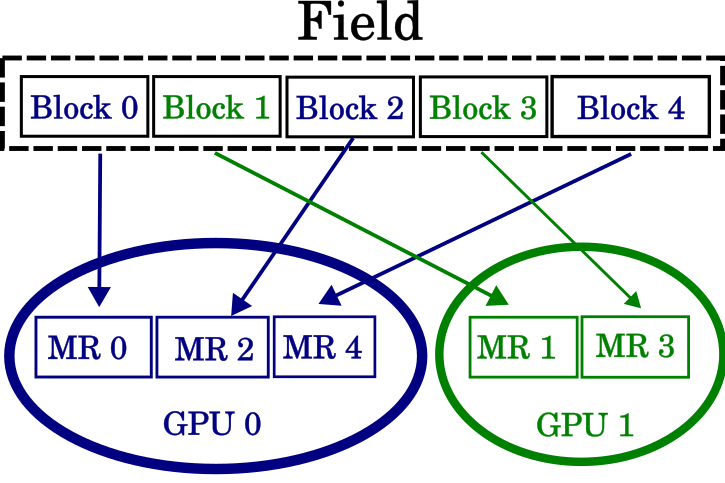
\includegraphics[width=1\textwidth]{./img/block-structure-1.png}
        \par\end{centering}
    \centering{}\caption{One \lstinline[style=C++Style]!MemoryRegion! per block} \label{fig:block-structure-1}
  \end{figure}
  
  \begin{figure}[htbp!]
    \begin{centering}
        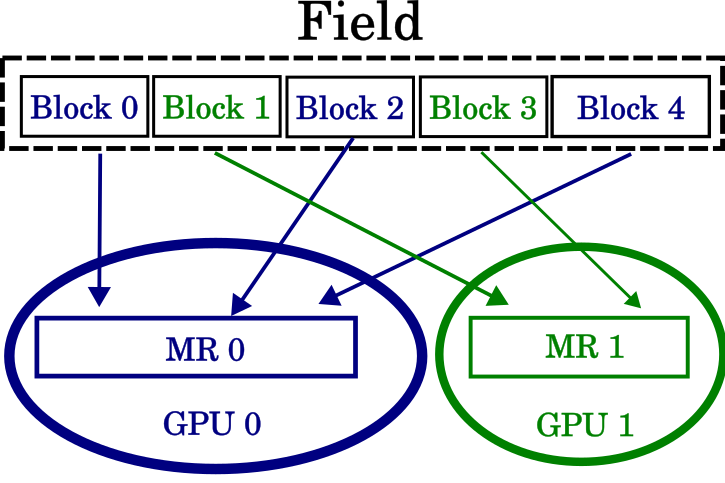
\includegraphics[width=1\textwidth]{./img/block-structure-2.png}
        \par\end{centering}
    \centering{}\caption{One \lstinline[style=C++Style]!MemoryRegion! per compute unit} \label{fig:block-structure-2}
  \end{figure}

  %\begin{figure}[htbp!]
  %  \begin{centering}
  %      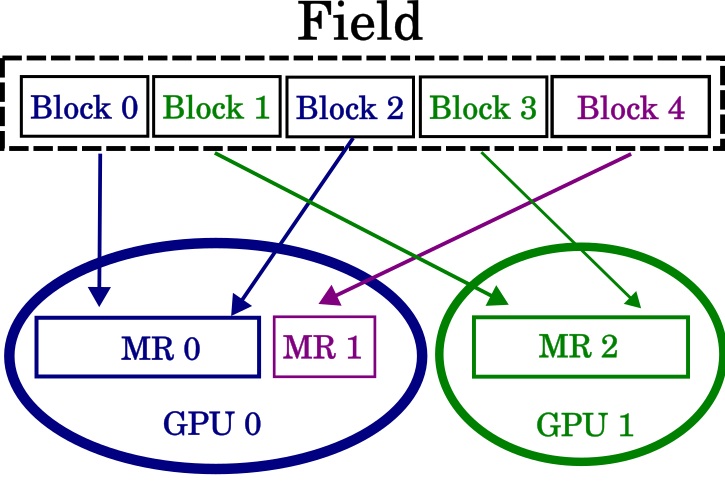
\includegraphics[width=1\textwidth]{./img/block-structure.png}
  %      \par\end{centering}
  %  \centering{}\caption{Unified design with generalized MemoryRegion mapping} \label{fig:block-structure}
  %\end{figure}

The mapping between the blocks and the \lstinline[style=C++Style]!MemoryRegion! objects is determined during the creation of the \lstinline[style=C++Style]!Field! object by the templated member function \lstinline[style=C++Style]!SetBlockToMemoryRegionMapping!. 
\begin{lstlisting}[style=C++Style]
template <typename MemSpace>
static void SetBlockToMemoryRegionMapping(
    Field<TData, TState> &field,
    const std::vector<BlockAttributes> blockAttr, const size_t alignment,
    const bool device_only = false)
{

#if defined(NEKTAR_USE_SINGLE_MEMORY_REGION_PER_DEVICE)
    std::vector<size_t> offset(field.m_num_device, 0);
    std::vector<size_t> size(field.m_num_device, 0);
    for (size_t blk = 0; blk < blockAttr.size(); ++blk)
    {
        // Set one-to-one MemoryRegion to device mapping.
        auto mr    = blk % field.m_num_device;
        auto nsize = blockAttr[blk].size() * field.GetNumComponents();
        field.m_blk_to_mr_mapping.push_back(mr);
        field.m_blk_to_mr_offset.push_back(offset[mr]);
        offset[mr] += nsize;

        // Compute MemoryRegion memory size.
        size[mr] += nsize;
    }
    for (size_t mr = 0; mr < field.m_num_device; ++mr)
    {
        // Allocate memory.
        auto device_rank = mr;
        field.m_memory_regions.push_back(
            MemoryRegion<TData>::template Create<MemSpace>(
                field.m_name + std::to_string(mr), size[mr], alignment,
                device_only, device_rank));

        // Zero memory.
        field.m_memory_regions[mr].template Initialize<MemSpace>(0);
    }
#else
    for (size_t blk = 0; blk < blockAttr.size(); ++blk)
    {
        // Set one-to-one block to MemoryRegion mapping.
        field.m_blk_to_mr_mapping.push_back(blk);
        field.m_blk_to_mr_offset.push_back(0);

        // Allocate memory.
        auto device_rank = blk % field.m_num_device;
        auto size        = blockAttr[blk].size() * field.GetNumComponents();
        field.m_memory_regions.push_back(
            MemoryRegion<TData>::template Create<MemSpace>(
                field.m_name + std::to_string(blk), size, alignment,
                device_only, device_rank));

        // Zero memory.
        field.m_memory_regions[blk].template Initialize<MemSpace>(0);
    }
#endif
    for (size_t blk = 0; blk < blockAttr.size(); ++blk)
    {
        field.m_block_accessors.push_back(BlockAccessor(
            blockAttr[blk],
            field.m_memory_regions[field.m_blk_to_mr_mapping[blk]],
            field.m_blk_to_mr_offset[blk]));
    }
}
\end{lstlisting}

The default implementation is the one \lstinline[style=C++Style]!MemoryRegion! per block mapping. The one \lstinline[style=C++Style]!MemoryRegion! per compute unit mapping can be enable using the follow cmake command
\begin{lstlisting}[style=BashInputStyle]
cmake ../ NEKTAR_USE_SINGLE_MEMORY_REGION_PER_DEVICE=ON
\end{lstlisting}

